\documentclass[tikz]{standalone}
\usetikzlibrary{chains}
\makeatletter
\tikzset{west below/.code=\tikz@lib@place@handle@{#1}{north west}{0}{-1}{south west}{1}}
\makeatother
\tikzset{
  typnode/.style={anchor=north west, text width=12cm, inner sep=0mm},
  data/.style={draw=gray, rectangle, font=\scriptsize, inner sep=0.5mm},
}
\begin{document}\footnotesize
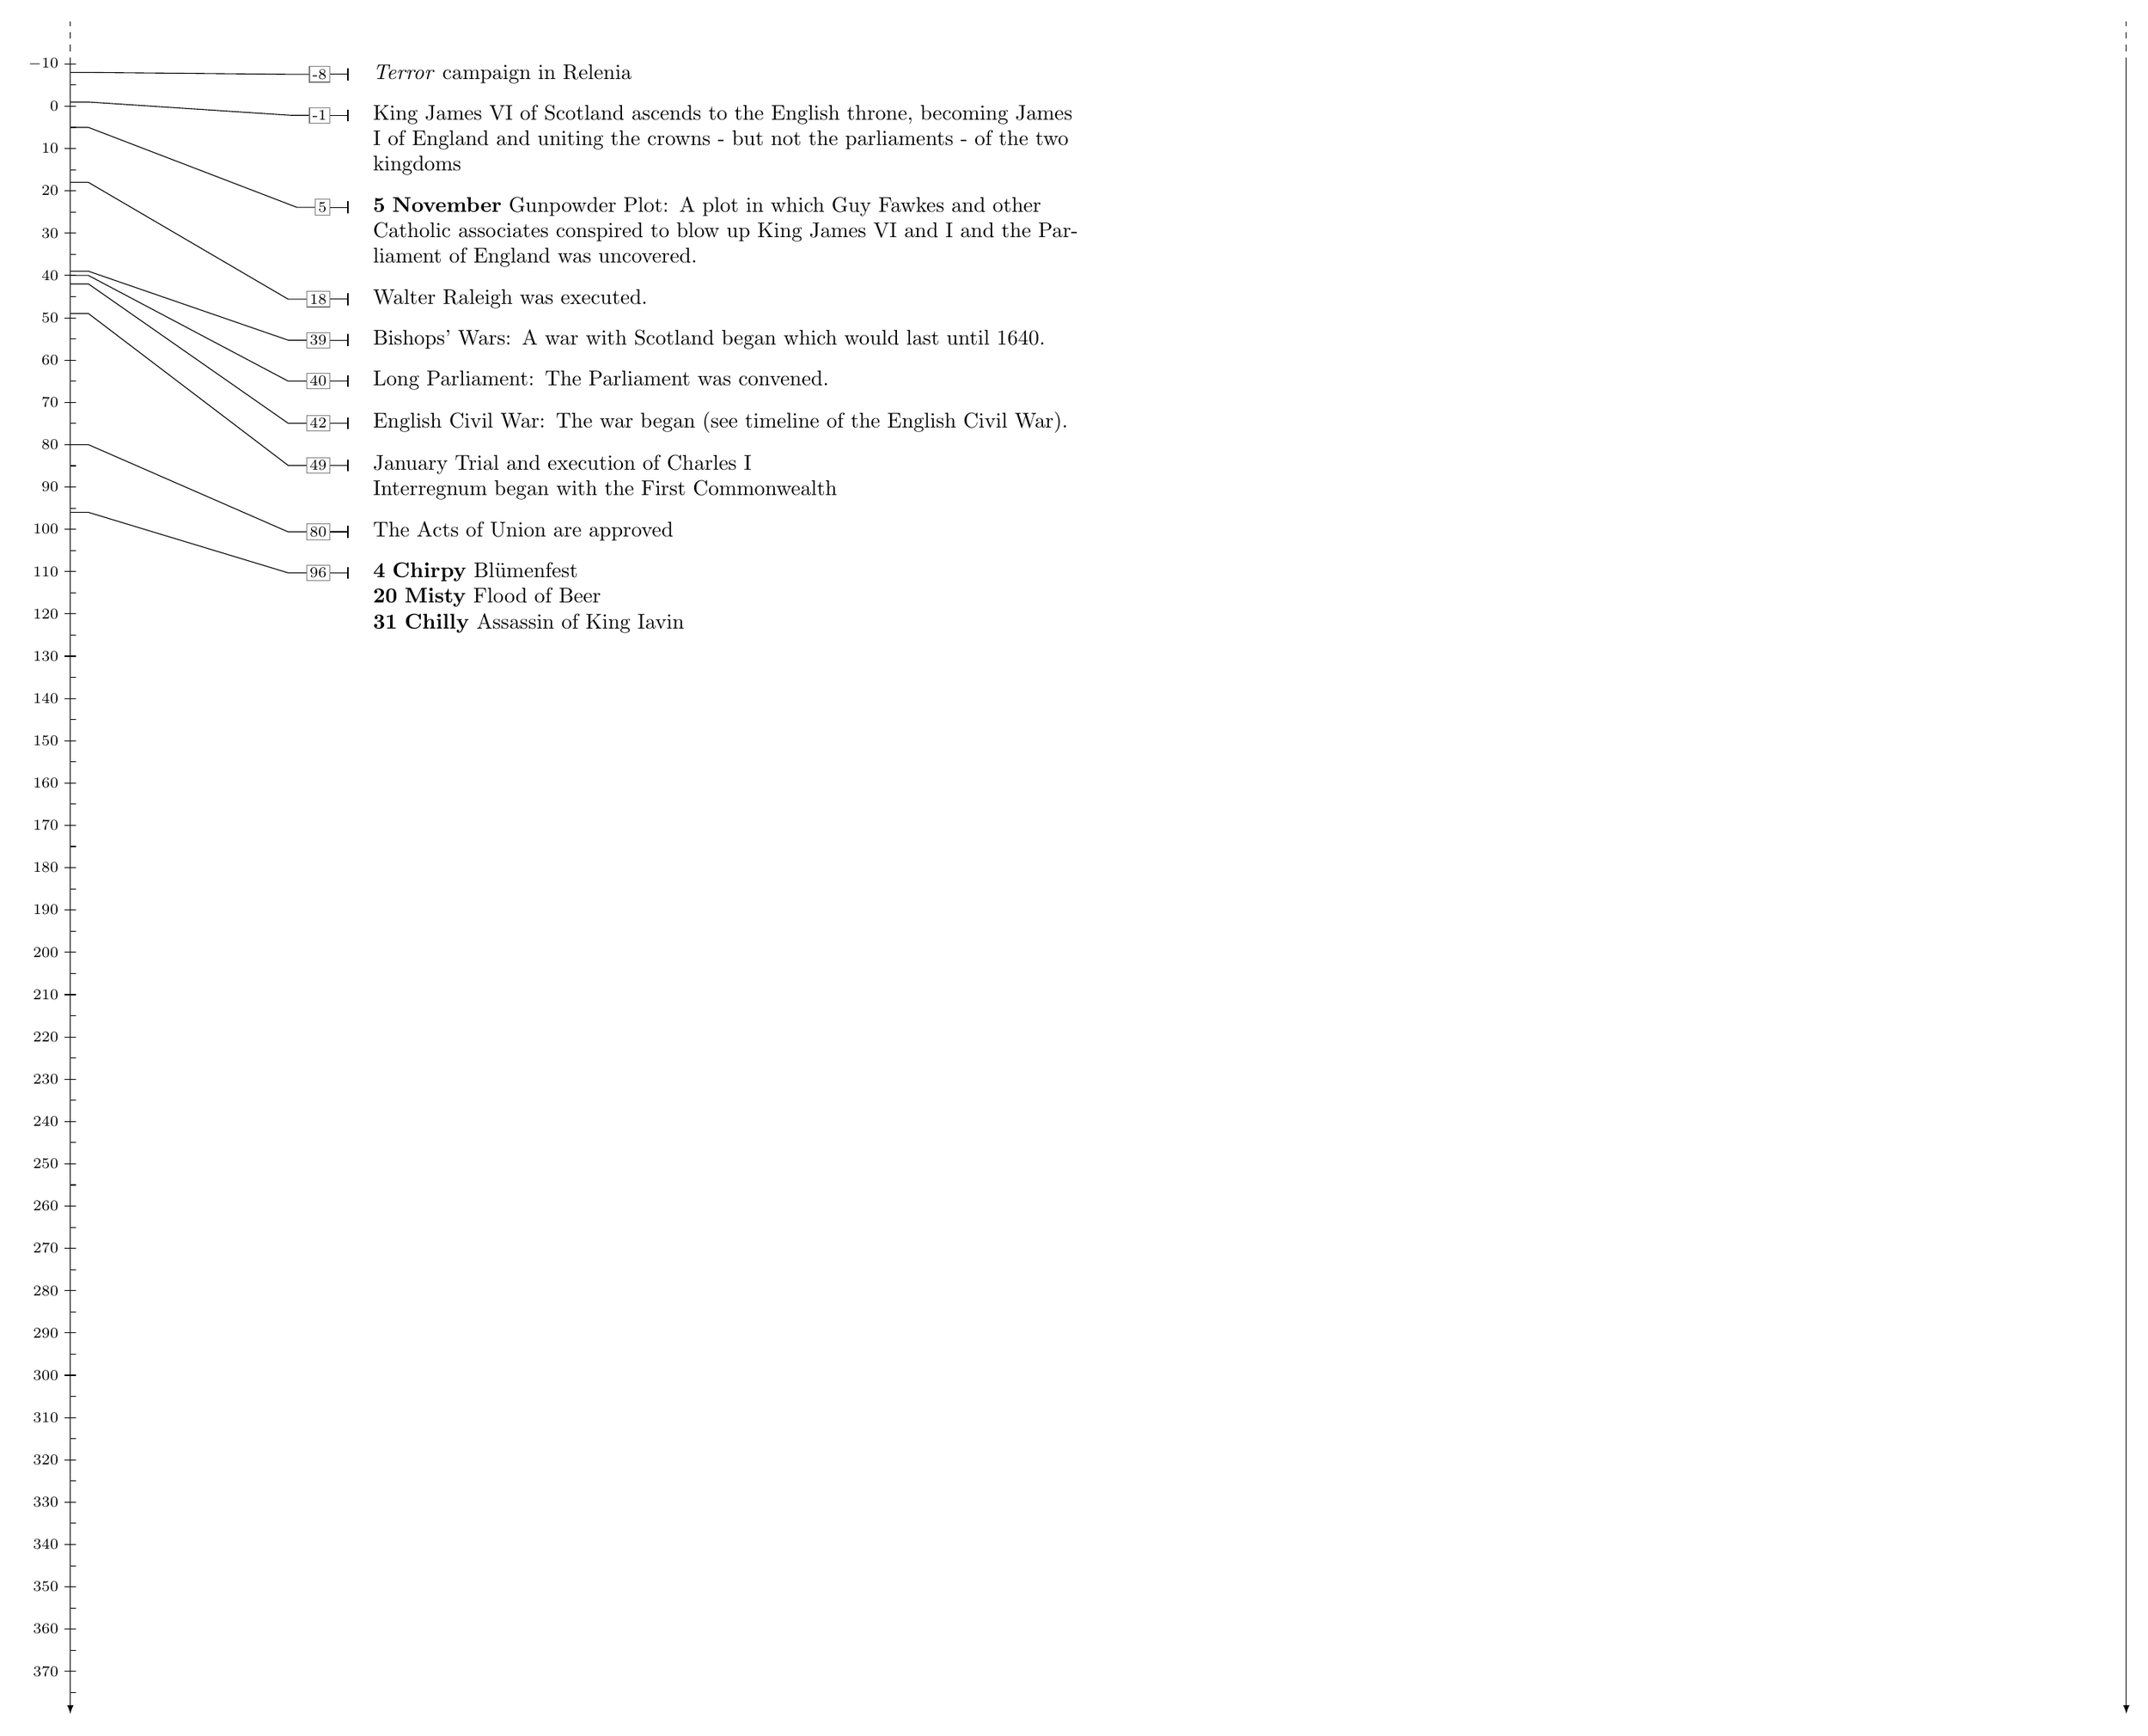
\begin{tikzpicture}[x=1cm, y=-7mm]
%draw horizontal line
\foreach \xValue in {0,34}
  \path (\xValue,0) edge[-latex] ++(0,39)
                    edge[dashed] ++ (down:1);

%%draw years													%% anno X=-10 da cui inziare a disegnare N=38 date distanti Y=10	
\foreach \y [evaluate=\y as \xear using int(-10+\y*10)] in {0,1,...,38}{  
  \node[left=2pt,anchor=east,xshift=0,font=\scriptsize] at (0,\y) {$\xear$}; 
  \draw (-0.1,\y) -- (0.1,\y); \draw (0,\y+.5) -- (0.1,\y+.5);
}

\begin{scope}[start chain=ch1 going west below, node distance=+1em]
\foreach \Year/\Text in {%
	 -8/{\textit{Terror} campaign in Relenia},             %% assicurarsi che questo anno sia >= X
     -1/{King James VI of Scotland ascends to the English throne, becoming James I of England and uniting the crowns - but not the parliaments - of the two kingdoms},
     5/{\textbf{5 November} Gunpowder Plot: A plot in which Guy Fawkes and other Catholic associates conspired to blow up King James VI and I and the Parliament of England was uncovered.},
     18/{Walter Raleigh was executed.},
     39/{Bishops' Wars: A war with Scotland began which would last until 1640.},
     40/{Long Parliament: The Parliament was convened.},
     42/{English Civil War: The war began (see timeline of the English Civil War).},
     49/{January Trial and execution of Charles I\\Interregnum began with the First Commonwealth},
     80/{The Acts of Union are approved},
     96/{\textbf{4 Chirpy} Bl\"{u}menfest \\ \textbf{20 Misty} Flood of Beer\\ \textbf{31 Chilly} Assassin of King Iavin} 
    %% WARNING: penultimo termina con , %% ultimo termina senza , %% no linea vuota tra ultimo e { 	
    }{
  \node[typnode, at=(right:5cm), on chain=ch1, alias=Text] {\Text};
  \node[data,    base left=+2em of Text, alias=Year] {\Year};
  \draw[-|] (Year.east) -- ++(right:3mm);
  \draw     (Year.west) -- ++(left:3mm)
                        -- ([shift=(right:3mm)] 0,{(\Year+10)/10})	%% ( \Year - (X) ) / Y
                        --                     (0,{(\Year+10)/10}); }

\end{scope}
\end{tikzpicture}
\end{document}